\documentclass[10pt,letterpaper]{article}
\usepackage[top=0.85in,left=1.75in,footskip=0.75in]{geometry}

% Use adjustwidth environment to exceed column width (see example table in text)
\usepackage{changepage}

% Use Unicode characters when possible
\usepackage[utf8x]{inputenc}

% textcomp package and marvosym package for additional characters
\usepackage{textcomp,marvosym}

% fixltx2e package for \textsubscript
\usepackage{fixltx2e}

% amsmath and amssymb packages, useful for mathematical formulas and symbols
\usepackage{amsmath,amssymb}

% cite package, to clean up citations in the main text. Do not remove.
\usepackage{cite}

% Use nameref to cite supporting information files (see Supporting Information section for more info)
\usepackage{nameref,hyperref}

% line numbers
\usepackage[right]{lineno}

% ligatures disabled
\usepackage{microtype}
\DisableLigatures[f]{encoding = *, family = * }

% Remove comment for double spacing
\usepackage{setspace} 
\doublespacing

% Text layout
\raggedright
\setlength{\parindent}{0.5cm}
\textwidth 5.25in 
\textheight 8.75in

% Bold the 'Figure #' in the caption and separate it from the title/caption with a period
% Captions will be left justified
\usepackage[aboveskip=1pt,labelfont=bf,labelsep=period,justification=raggedright,singlelinecheck=off]{caption}
\renewcommand{\figurename}{Fig}

% Use the PLoS provided BiBTeX style
\bibliographystyle{plos2015}

% Remove brackets from numbering in List of References
\makeatletter
\renewcommand{\@biblabel}[1]{\quad#1.}
\makeatother

% Leave date blank
\date{}

% Header and Footer with logo
\usepackage{lastpage,fancyhdr,graphicx}
\usepackage{epstopdf}

%% Include all macros below
\newcommand{\khalf}{\left(\frac{1}{2}\right)^{\delta_{ij}}}  % (1/2)^kronecker
\newcommand{\kkhalf}{\left(\frac{1}{2}\right)^{\delta_{ij} \delta_{kl}}}  % (1/2)^(kronecker * kronecker)
\newcommand{\Lspvl}{$\log_{10}$ SPVL}
\newcommand{\rzero}{{\mathcal R}_0}
\newcommand{\etal}{\textit{et al.}}
\newcommand{\tsub}[2]{#1_{{\textrm{\tiny #2}}}}
\newcommand{\PF}{\textrm{PF}}
\newcommand{\DS}{\textrm{DS}}
\newcommand{\WT}{\textrm{WT}}
\newcommand{\ET}{\textrm{ET}}
\newcommand{\DM}{\textrm{DM}}

\newcommand{\todo}[1]{\textbf{#1}}

\renewcommand\thefigure{\Alph{figure}}    

%% END MACROS SECTION

\begin{document}

\section*{Supporting Information S2: dynamics of transmission and virulence}

This section presents alternate versions of
the figures from the main text showing time dynamics and summary
statistics in terms of expected progression time to AIDS and per-year transmission probability
rather than \Lspvl.

\begin{figure}[!ht]
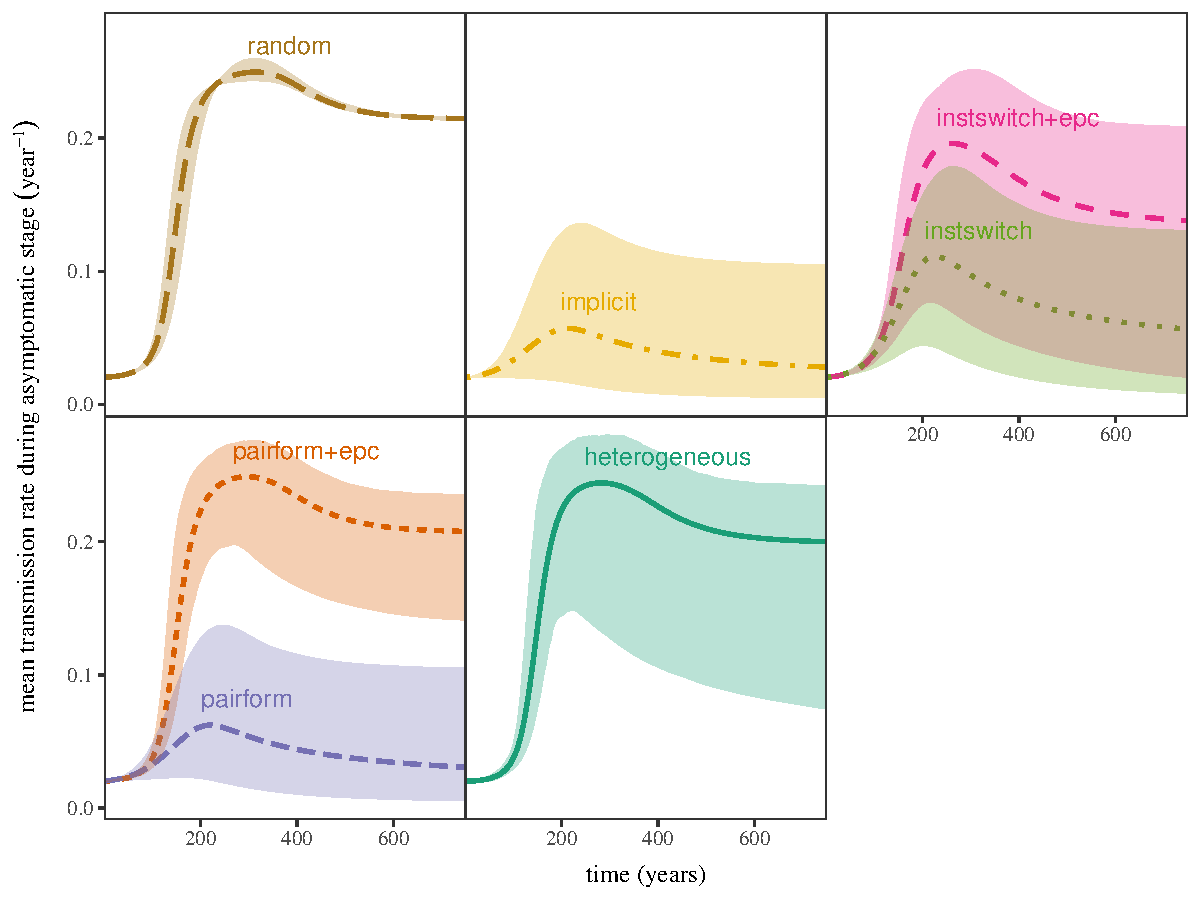
\includegraphics[width=\textwidth]{../figures/fig_S2_1.pdf}
\caption{{\bf Envelopes of transmission trajectories under all models.}
This figure matches Fig 3 in main text, but displays the
envelope of population-mean transmission probabilities rather than mean \Lspvl\ over time
for each model.
}
\label{fig:transtraj}
\end{figure}

\clearpage

\begin{figure}[!ht]
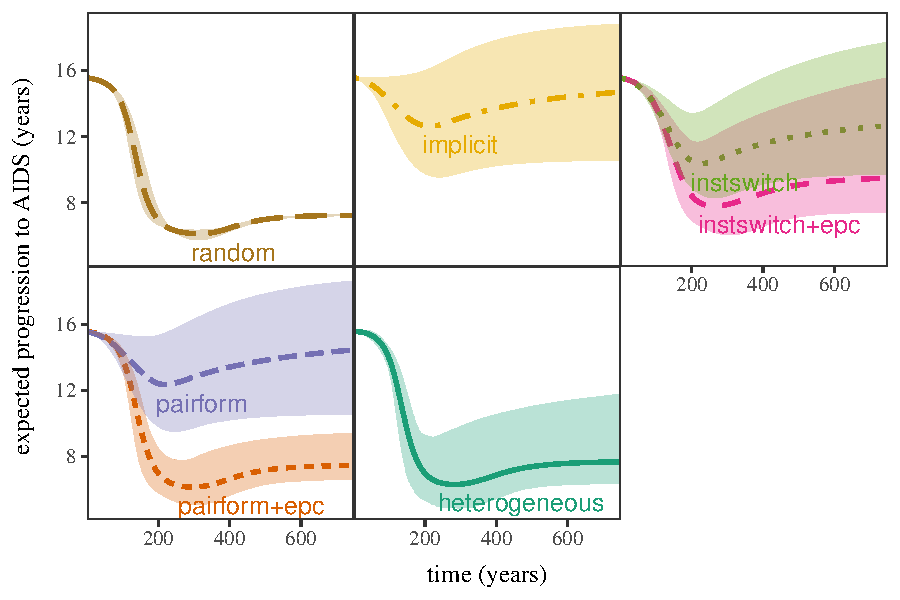
\includegraphics[width=\textwidth]{../figures/fig_S2_2.pdf}
\caption{{\bf Envelopes of expected progression time to AIDS trajectories under all models.}
This figure matches Fig 3 in main text, but displays the
envelope of expected progression time to AIDS rather than mean \Lspvl\ over time
for each model.
}
\label{fig:durtraj}
\end{figure}

\clearpage

%% \Lspvl\ doesn't get bolded so I got rid of log10
\begin{figure}[!ht]
  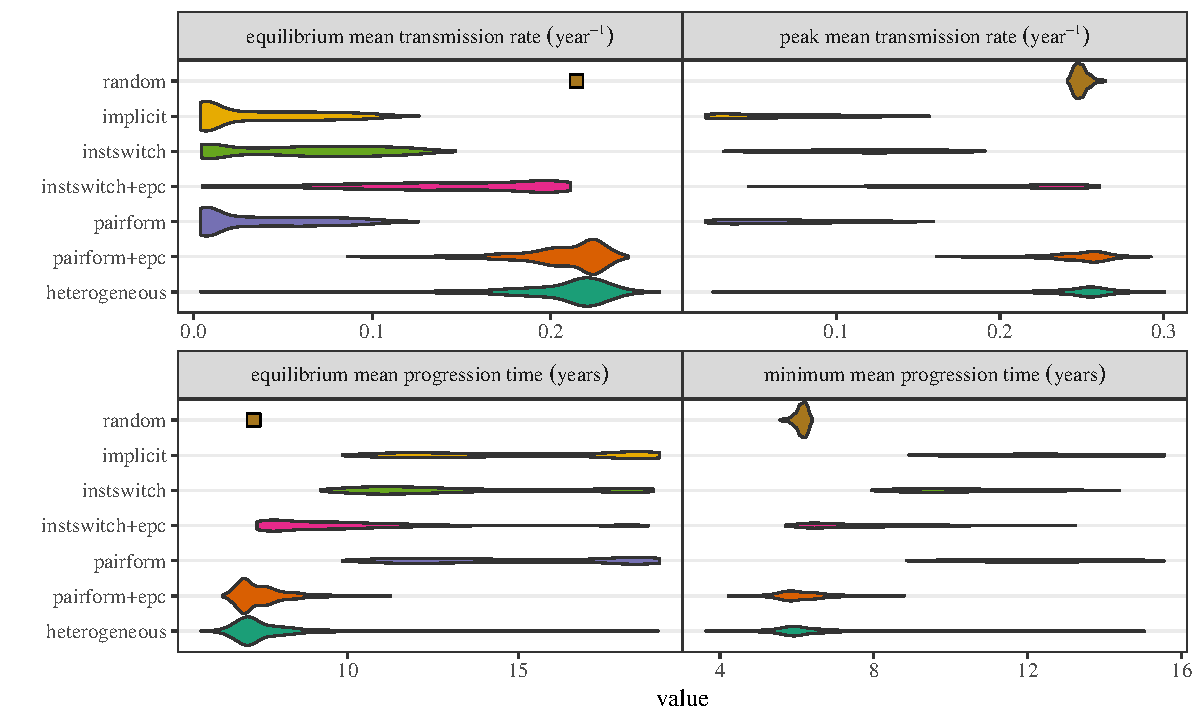
\includegraphics[width=\textwidth]{../figures/fig_S2_3.pdf}
\caption{{\bf Univariate distributions of transmission probabilities and expected progression time to AIDS.}
This figure matches Fig 4 in main text, but displays the
univariate distributions for the transmission probability and expected progression time to AIDS time at the virulence
peak and at the epidemiological equilibrium,
rather than the distributions of \Lspvl.
}
\label{fig:trandursum}
\end{figure}

\clearpage

\begin{figure}[!ht]
  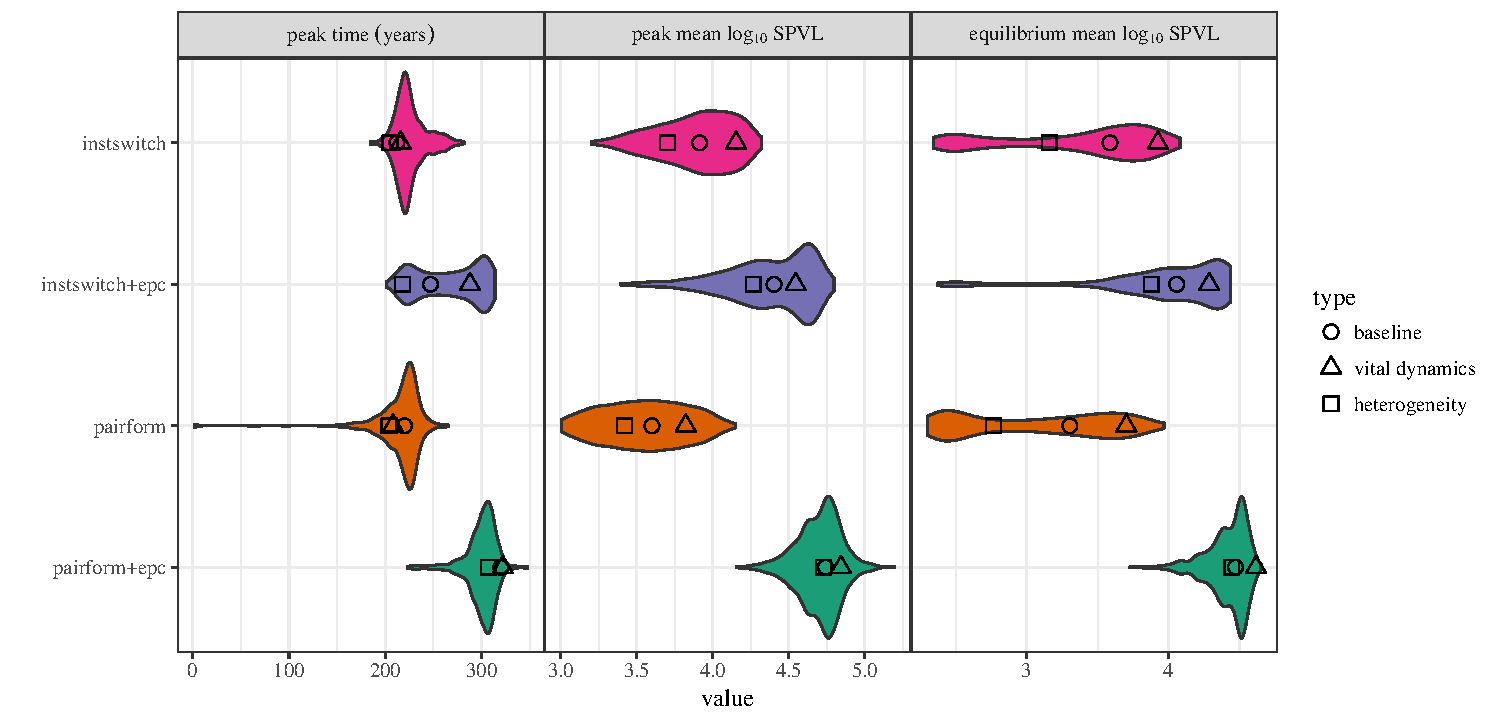
\includegraphics[width=\textwidth]{../figures/fig_S2_4.pdf}
\caption{{\bf Effects of contact heterogeneity and vital dynamics.}
This figure matches Fig 4 in main text, but adds results
for model variants with contact heterogeneity and vital dynamics.
The violin plots, copied from Fig 4 in the main text, show the
distribution of outcomes across the Latin hypercube sample
for SIS model without contact heterogeneity. The points show
the outcome of various models using the baseline parameters
from Table 1: (\emph{circle}) unmodified 
models (SIS, homogeneous); (\emph{triangle}) models with vital dynamics; 
(\emph{square}) models with contact heterogeneity.
}
\label{fig:fig3aug}
\end{figure}

\end{document}
